\documentclass[aspectratio=169]{beamer}
\usepackage[utf8]{inputenc}

\setbeamersize{text margin left=3mm,text margin right=3mm} 

\usetheme{Oxygen}
\usepackage{graphicx}
\usepackage{hyperref}
%\usepackage{movie15}
\usepackage{textpos}
\usepackage{fancybox}
\usepackage{colortbl}
\usepackage{rotating}
\usepackage{subfigure}
%\usepackage{subcaption}
\usepackage{multicol}
\usepackage{multirow}
\usepackage{amsmath,amssymb,amsfonts,amsbsy,dsfont}
\usepackage{mathrsfs}
\usepackage{amsthm}
\usepackage{bm}
\usepackage{array}
%\usepackage[caption=false]{subfig}
\usepackage{arydshln}

\let\oldcite\cite % store the original \cite command
\renewcommand{\cite}[1]{{\tiny\oldcite{#1}}}

\usepackage{bm}
\providecommand{\mat}[1]{{\bm{#1}}} 
\providecommand{\ve}[1]{{\bm{#1}}} 


\newcommand{\x}{\negthinspace\times\negthinspace}
\usepackage{etoolbox}


\usepackage[nopar]{lipsum} 

\newif\ifcomment
\newcommand{\Com}{\par\footnotesize\itshape\commenttrue}

\newenvironment{Itemize}
 {%
  \edef\Itemizecurrent{\the\font}%
  \itemize
  \preto{\item}{\ifcomment\par\Itemizecurrent\fi}%
 }{%
  \enditemize
 }


%%%%%%%%%%%%%%%%%%%%%%%%%%%%%%%%%%%%%%%%%%%%%%%%%%%%%%
%%%%%%%


\title[LPAR 2023 | Foot Segmentation for Regional Analgesia Monitoring using Convolutional Random Fourier Features]{Foot Segmentation for Regional Analgesia Monitoring using Convolutional Random Fourier Features}
\author{J.~Aguirre-Arango\inst{1} \and A.~{A}lvarez-Meza\inst{1} \and G.~Castellanos-Dominguez\inst{1}
}

\institute{
\inst{1}Signal~Processing~and~Recognition~Group,~Universidad~Nacional~de~Colombia, Manizales,~Colombia. \\
\{jucaguirrear,amalvarezme,cgcastellanosd\}@unal.edu.co
\\

\includegraphics[width=0.15\textwidth]{EscudoUN.png}
}

% \institute{
\includegraphics[width=0.15\textwidth]{EscudoUN.png}\\\footnotesize{
% Universidad Nacional de Colombia \\ Signal Processing and Recognition Group - SPRG
% \\
% Advisor: Andrés Marino Álvarez Meza, Ph.D.\\

% }}
\date[]{\footnotesize{\today \\ LPAR 2023: 24th International Conference on Logic for Programming, Artificial Intelligence and Reasoning}}
%%-------------------------------------------------------------------
%% Options
%%-------------------------------------------------------------------
\setbeamercovered{dynamic}
\setbeamertemplate{navigation symbols}{}



\begin{document}

{\setbeamertemplate{headline}{}
\setbeamertemplate{footline}{}
\begin{frame}{}
\vspace{-0.7cm}
    \titlepage 
\end{frame}
}


\frame
{ \frametitle{Outline}
{\small 
  \tableofcontents[]}
}

\AtBeginSection[]
{
  \begin{frame}
  \frametitle{Outline}
  \tableofcontents[currentsection]
  \end{frame}
}



%%%%%%%%%%%%%%%%%%%%%%%%%%%%%%%%%%%%%%%%%
\section[Motivation]{Motivation and Problem}

\begin{frame}[allowframebreaks]{Childbirth pain monitoring}
    
Childbirth is one of the most painful events {\tiny{\cite{WOS:000754419000014}}}.


\begin{columns}
\column{0.5\textwidth}
\begin{figure}
    \centering
    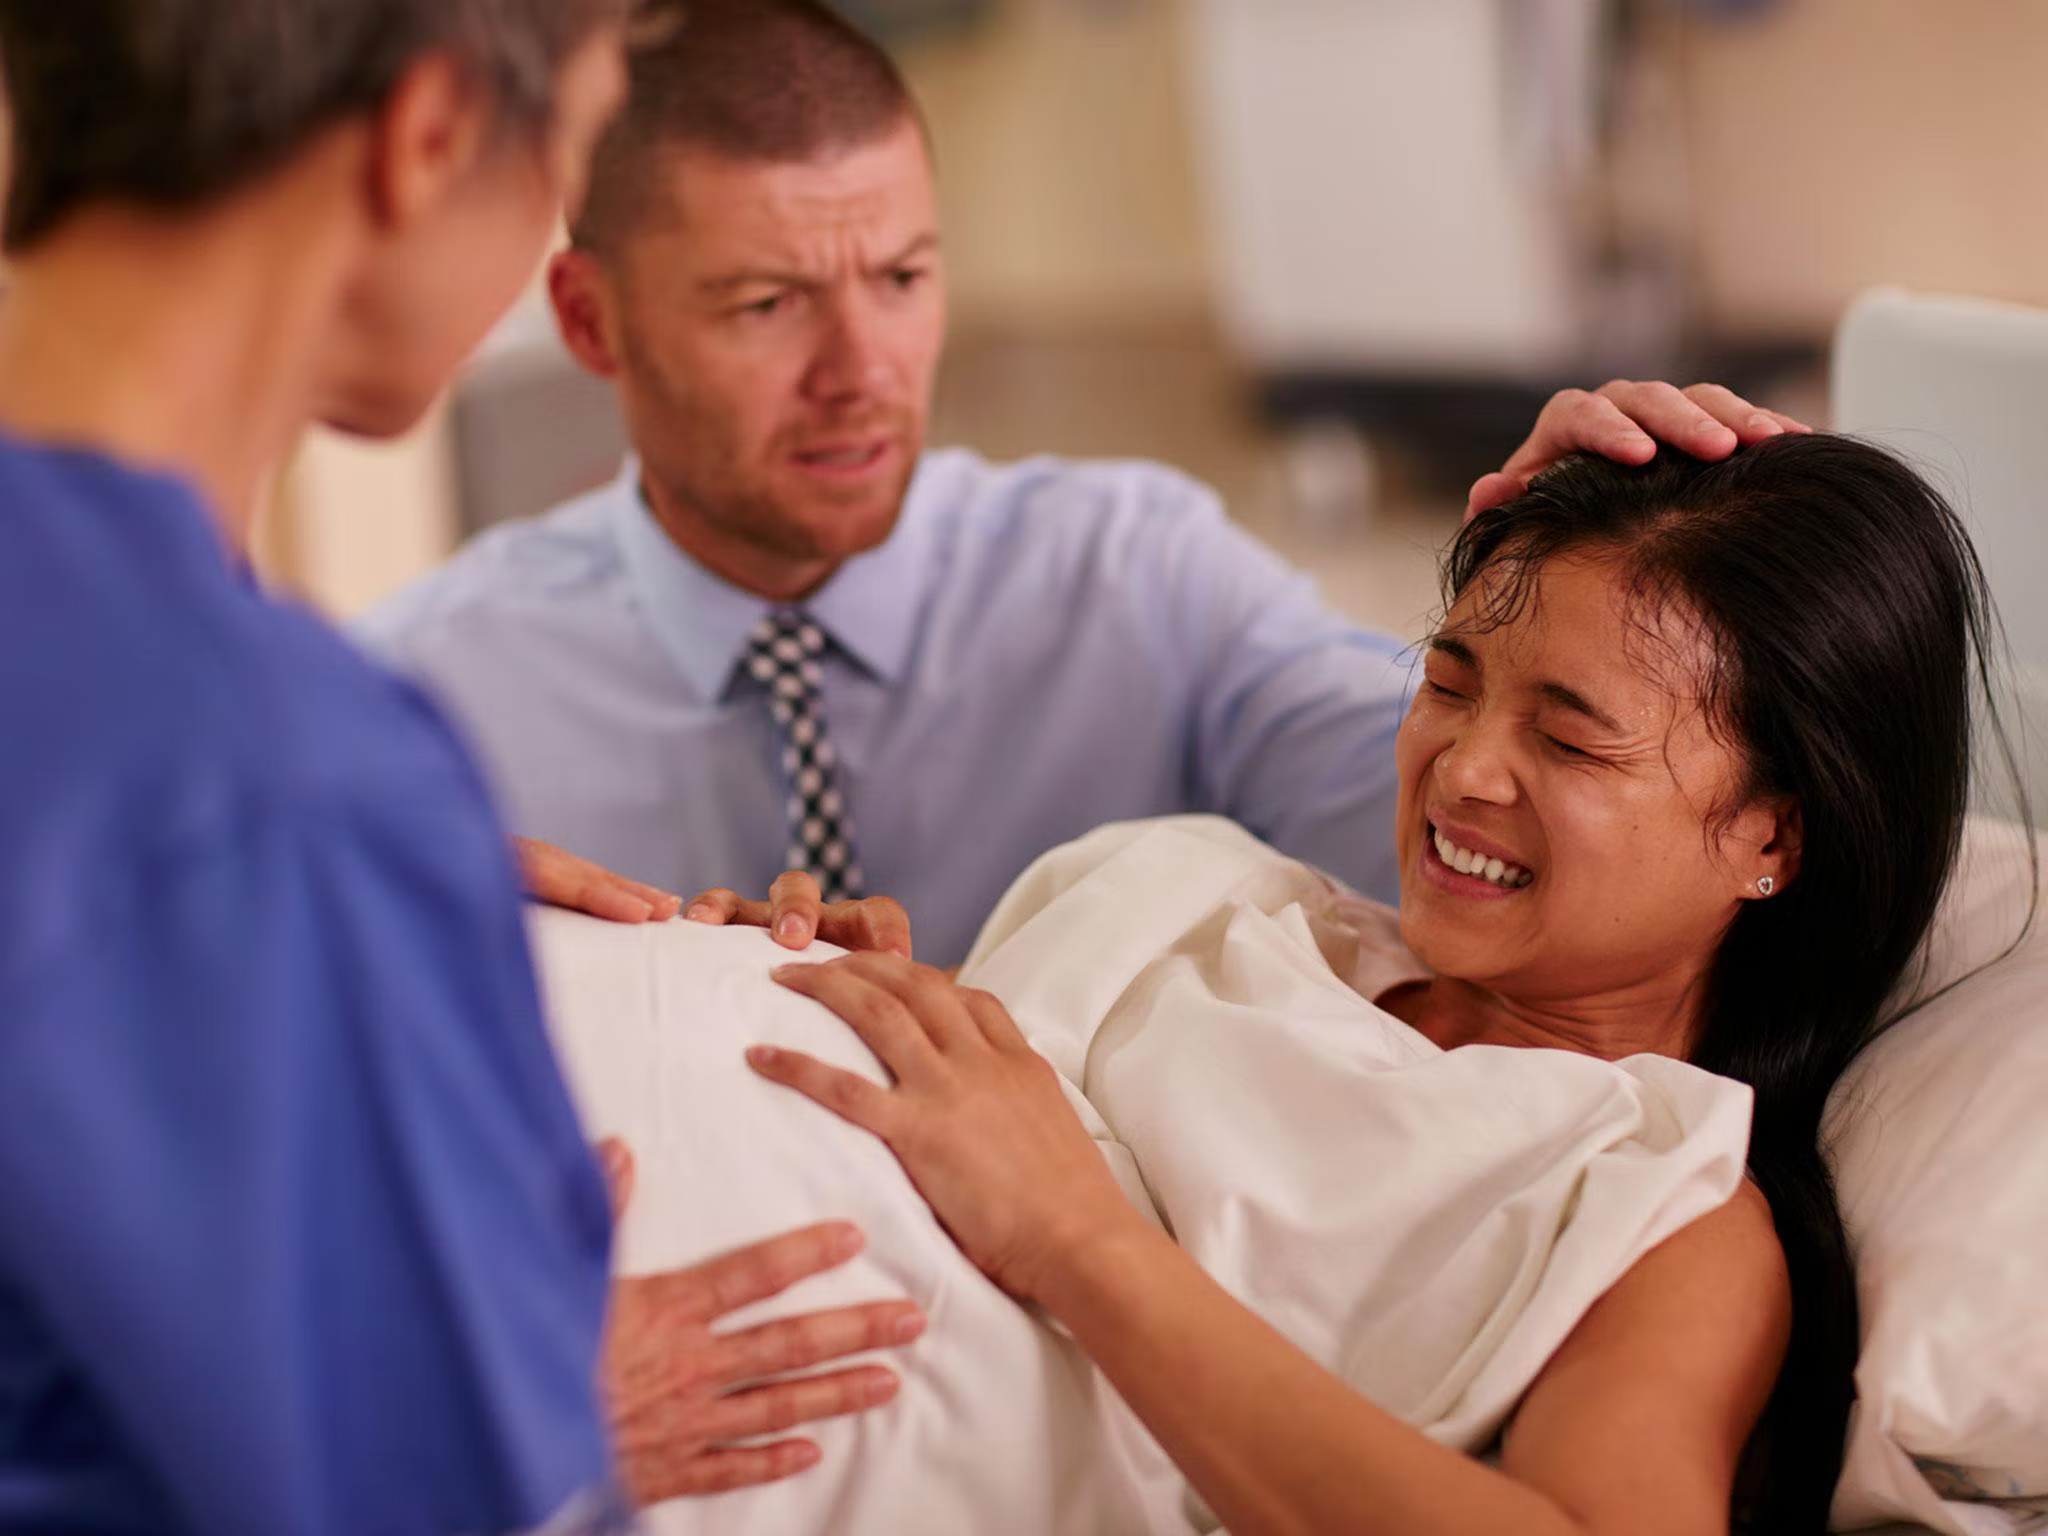
\includegraphics[width=0.8\linewidth]{Figures/labour.png}
\end{figure}

\column{0.5\textwidth}
\centering
{\color{blue} 
Regional neuraxial analgesia is one of the safest methods for pain relief {\tiny{\cite{WOS:000613005100038}}}. 
}
\end{columns}


\framebreak

\begin{figure}
    \begin{subfigure}
        \centering
        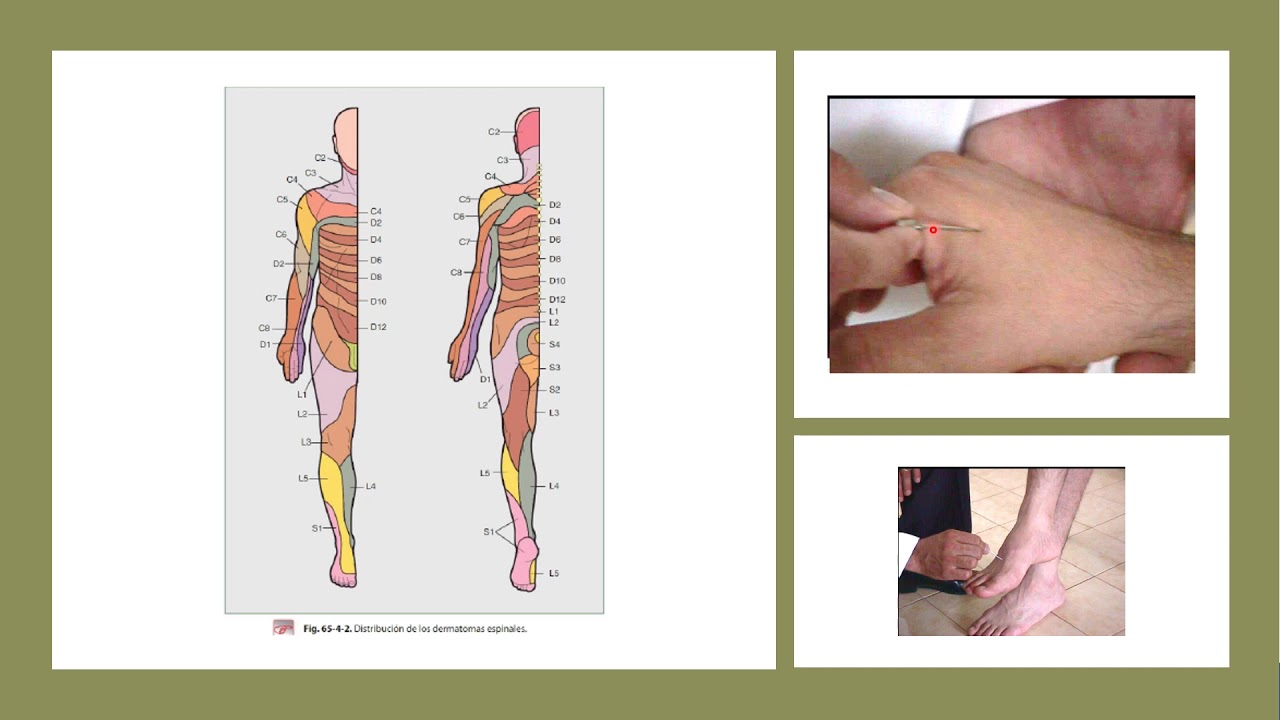
\includegraphics[height = 0.2\textwidth]{Figures/termoalgesia.jpg}
        \label{fig:termoalgesia}
    \end{subfigure}
    \begin{subfigure}
        \centering
        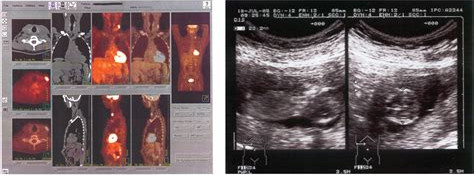
\includegraphics[height = 0.2\textwidth]{Figures/pet2.jpeg}
        \label{fig:pet2}
    \end{subfigure}
    \label{fig:pet}
    \caption{Standard techniques for pain monitoring.}
\end{figure}
\vspace{-0.5cm}
\begin{itemize}
    \item Sensory thermoalgesic tests {\cite{https://doi.org/10.1111/anae.12927}}.
    \item Electrophysiological modalities {\cite{CHAE2022104744}}.
    \item PET imaging techniques {\cite{nelson2018survey}}.
\end{itemize}

\begin{center}
\small{\textcolor{blue}{\textbf{Low-cost, non-invasive, and highly reliable techniques are required.} }}
\end{center}

\framebreak

Thermal imaging is an objective and non-invasive technique to quantify warm modifications after catheter placement due to blood flow redistribution~{\tiny{\cite{2143r23}}}. 

\begin{columns}
\column{0.5\textwidth}

\begin{figure}
    \centering
    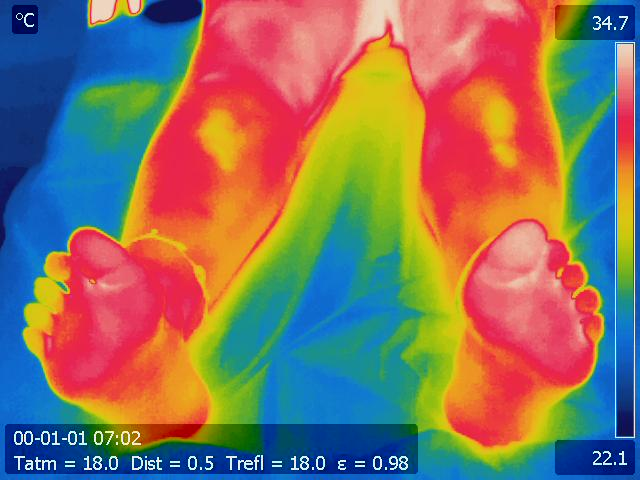
\includegraphics[width=0.8\linewidth]{Figures/t20rainbow.jpg}
    \caption{Thermal imaging example.}
\end{figure}


\column{0.5\textwidth}
%\textbf{A suitable assessment requires temperature measurements from the patient's feet soles taken at different position and times after the catheter placement to characterize the earlier thermal modifications.} \cite{5262452,PMID:19224821}


\textcolor{blue}{\textbf{Reliable and automatic thermal measurements are required during childbirth analgesia monitoring}} {\tiny{\cite{PMID:25232864}}}.


\end{columns}

\framebreak


\begin{itemize}
    \item Servicios Especiales de Salud (SES) Hospital Universitario de Caldas has high-quality health services.
    \item Objective and low-cost monitoring procedures for obstetric patients under regional neuraxial analgesia are still necessary.
\end{itemize}
 

\begin{figure}
    \centering
    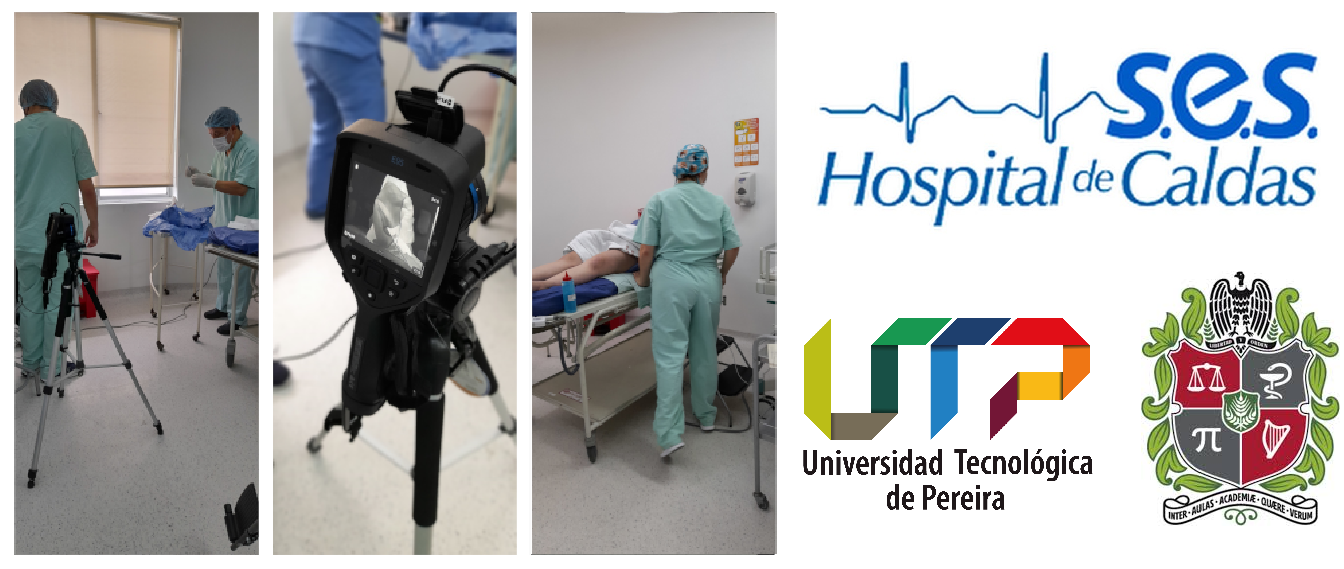
\includegraphics[width=0.7\linewidth]{Figures/ses_unal_utp.pdf}
    %\caption{Feet thermal image example.}
\end{figure}


\end{frame}

% \begin{frame}{Problems}


% \begin{itemize}
%     \item  \textbf{Small Sample Size and Overfitting}:
%     Difficulties in the adquisicion of datasets in obstetrics enviroments~\cite{WOS:000754419000014,willemink2020preparing}. Effectiveness heavily relies on extensively annotated datasets for training~\cite{sarker2021deep, li2021systematic}

%     \item \textbf{High Variability in the ROI in Medical Imaging}: Differences in anatomy, pathology, and imaging parameters, which can lead to significant variations in the ROI's shape, size, and texture \cite{li2021systematic}. Secondly, the high variability of foot positions can lead to images with different orientations, sizes, and shapes. This variability is often present even within the same subject, resulting in a wide range of foot positions, including cases where the feet may overlap or be partially obscured \cite{arteaga2021segmentation}

%     \item \textbf{Lack of quatitative measures for interpretabiity of semantic segmentation models}: black-box nature of SS models based on DL, their explainability is challenging \cite{linardatos2020explainable}. Most current methods for explainability on SS models rely mainly on visual inspection or qualitative analysis to evaluate the model's performance \cite{Wang_2022, salahuddin2022transparency}
% \end{itemize}
 
% \end{frame}



\begin{frame}{Small Sample Size and Overfitting}

\begin{itemize}
\setlength\itemsep{1em}
    \item Challenges in acquiring sufficient datasets in obstetrics environments \cite{WOS:000754419000014, willemink2020preparing}
    \item Effective training requires extensive annotations \cite{sarker2021deep, li2021systematic}.
\end{itemize}

\begin{figure}
    \centering
    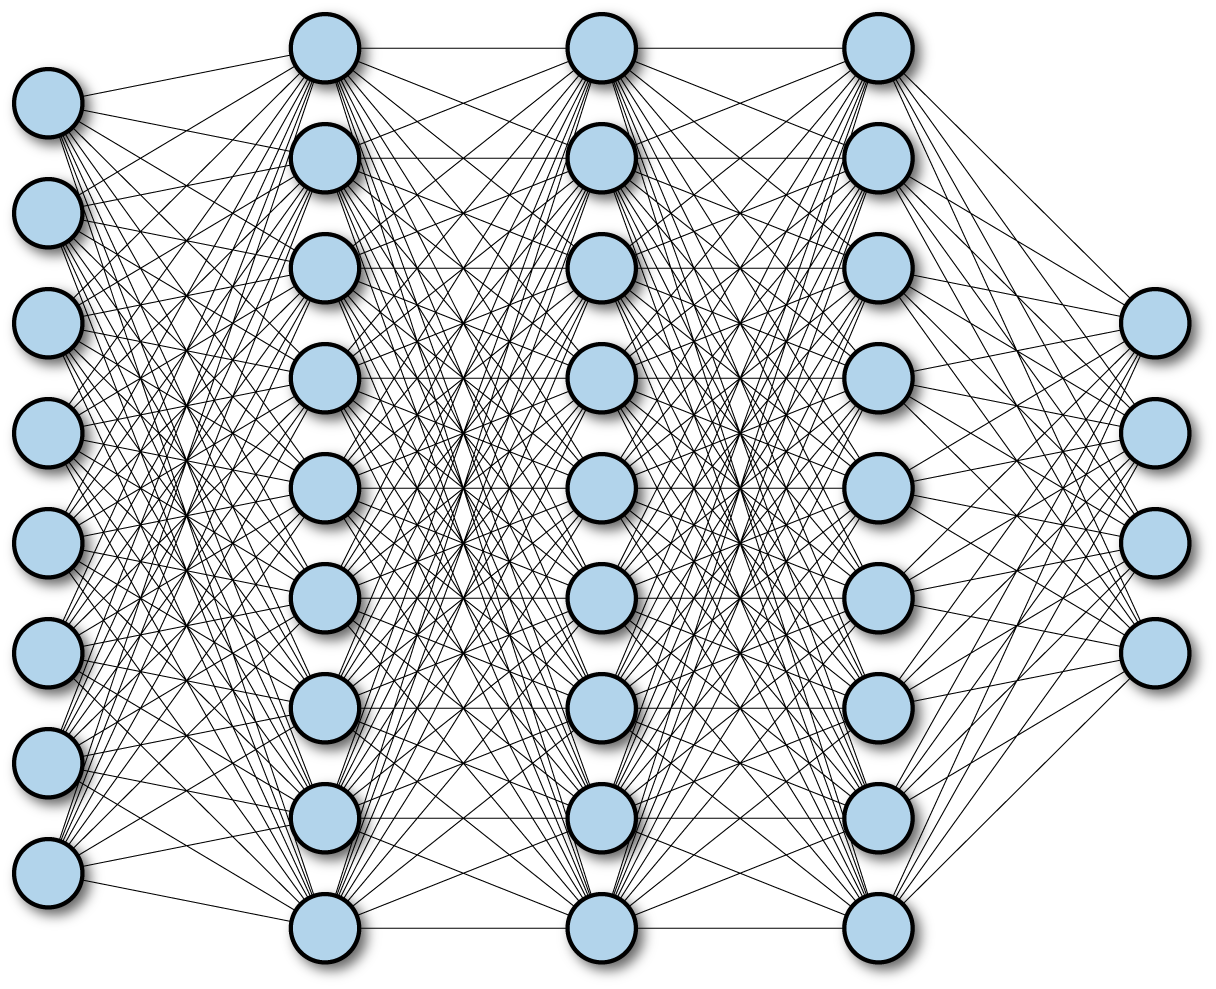
\includegraphics[width=0.4\textwidth]{overparametrized.png}
\end{figure}

\end{frame}


\begin{frame}{High Variability in the ROI in Medical Imaging}

\begin{itemize}
\setlength\itemsep{1em}
    \item Variations in anatomy, pathology, and imaging parameters result in significant variations in the Region of Interest's shape, size, and texture \cite{li2021systematic}.
    \item Diverse foot positions can lead to images with different orientations, sizes, and shapes, even within the same subject. This variability includes cases where the feet may overlap or be partially obscured \cite{arteaga2021segmentation}.
\end{itemize}
     
\begin{figure}
    \centering
    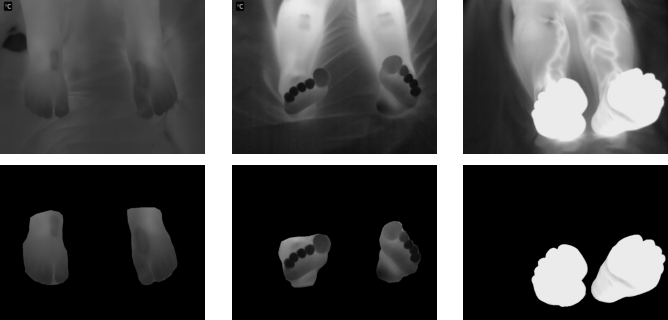
\includegraphics[width=0.5\textwidth]{Figures/high_roi_var.png}

\end{figure}

\end{frame}


\begin{frame}{Lack of Quantitative Measures for Interpretability of SS Models}

\begin{itemize}
\setlength\itemsep{1em}
    \item  Deep learning-based semantic segmentation models are often black-box, making their explanations challenging \cite{linardatos2020explainable}. 
    \item Current methods for explainability rely mainly on visual inspection or qualitative analysis, limiting the evaluation of model performance \cite{Wang_2022, salahuddin2022transparency}. 

    \begin{figure}
        \centering
        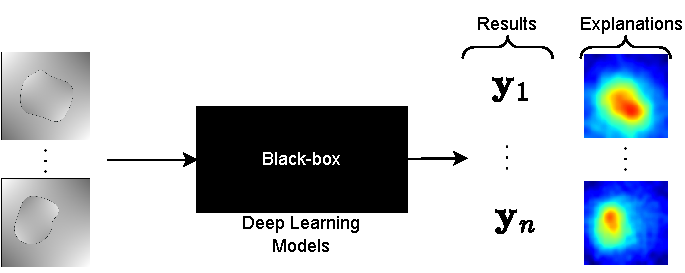
\includegraphics[width=0.61\textwidth]{Figures/lack_interpretability.pdf}
        
    \end{figure}
\end{itemize}

\end{frame}

\section{Literature Review}

\begin{frame}{Small Sample size and
Overfitting}

\begin{figure}
    \centering
    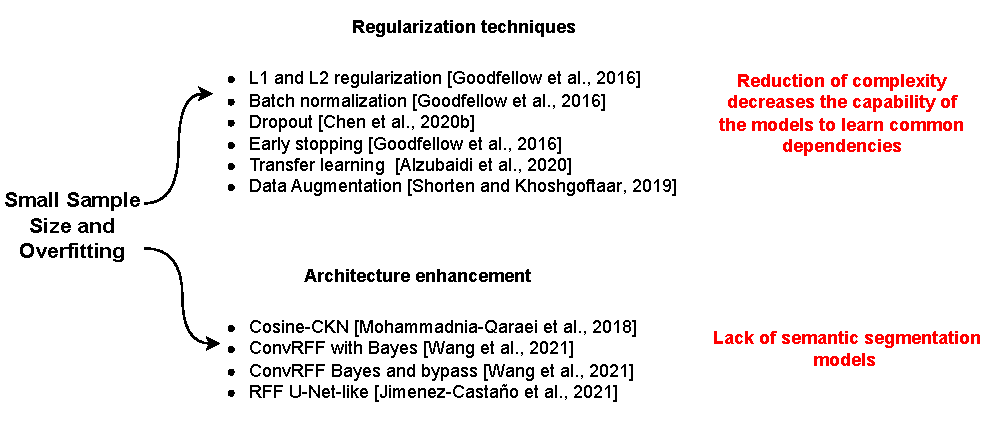
\includegraphics[width=0.8\linewidth]{Figures/State-of-the-arr-obj1.pdf}
    %\caption{Caption}
    %\label{fig:my_label}
\end{figure}   

\end{frame}

\begin{frame}{Characterization of
highly variable object patterns in CNN}
\begin{figure}
    \centering
    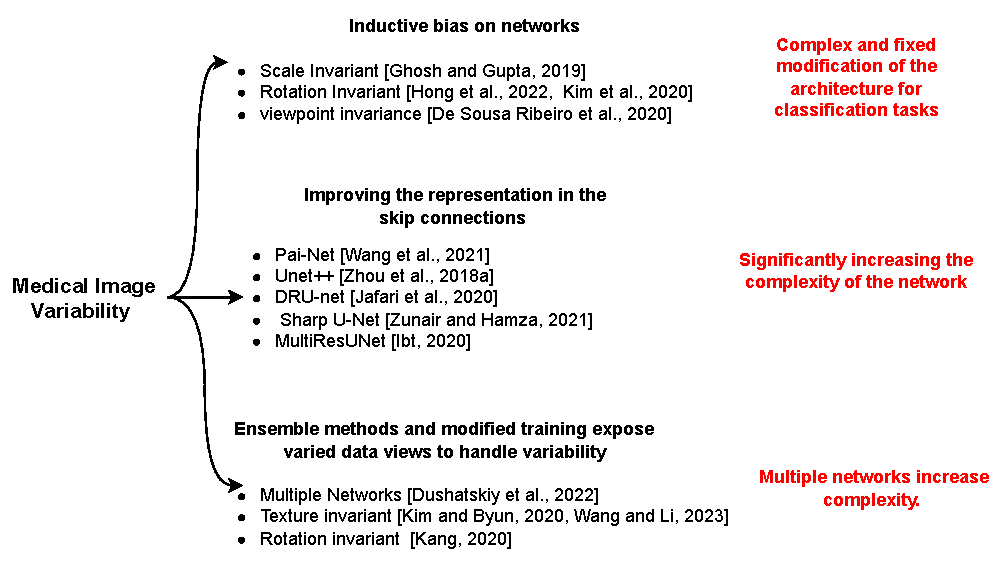
\includegraphics[width=0.8\linewidth]{Figures/State-of-the-ar-obj2.pdf}
    %\caption{Caption}
    %\label{fig:my_label}
\end{figure}    
\end{frame}


\begin{frame}{ Quantitative Interpretability of SS models}
\begin{figure}
    \centering
    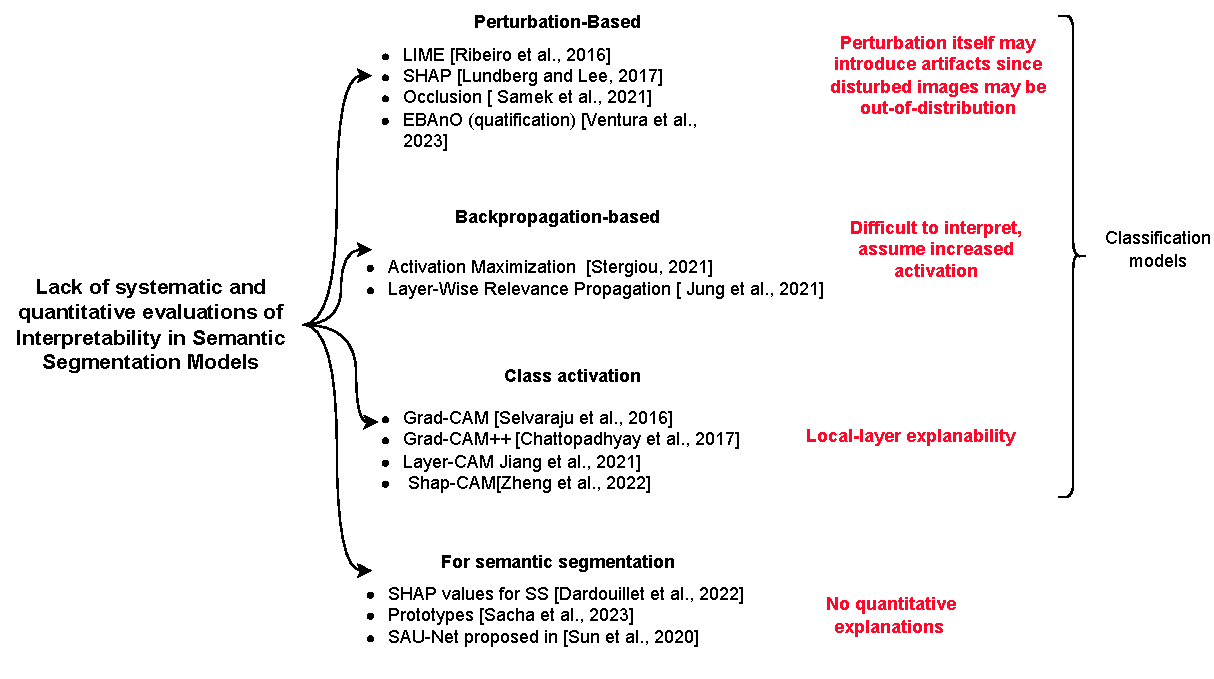
\includegraphics[width=0.8\linewidth]{Figures/State-of-the-ar-obj3.pdf}
    %\caption{Caption}
    %\label{fig:my_label}
\end{figure}    
\end{frame}


\section{Proposal}

\begin{frame}{Proposal}

\begin{figure}
    \centering 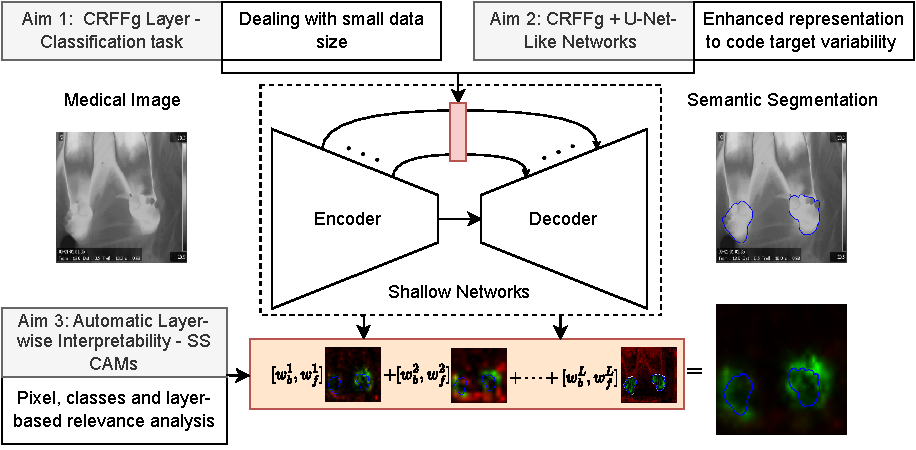
\includegraphics[width=0.8\linewidth]{Figures/contribution_thesis.pdf}
\end{figure}

\end{frame}

\begin{frame}{Mathematical Background}
    

\begin{itemize}
    \item \textbf{Dataset}: $$\{\mathbf{I}_n \in \mathbb{R}^{R \times C} , \mathbf{M}_n \in \{ 0, 1\} ^{R \times C} \s{:} n \in N\}$$
    $\mathbf{I}_n$ and $\mathbf{M}_n$ are the n-th image and target mask, respectively.
    \item \textbf{Model}: 
    $$\mathbf{\hat{M}} = (\varphi_L \circ \dotsb \circ \varphi_1)(\mathbf{I})$$
    $\varphi_l$ is  the $l$-th convolutional layer with parameters $\{\mathbf{W}_l \in \mathbb{R}^{P_l \times P_l \times D_l} : l \in L\}$.
    \item \textbf{Dice-based optimization problem}:
    $$
	 \{\mathbf{W}_l\}^L_{l=1} = \arg\min_{\mathbf{W}_l}
		 -2 \frac{\mat{1}^\top(\mat{M}_n \odot \mat{\hat{M}}_n)\mat{1} + \epsilon}{\mat{1}^\top \mat{M}_n\mat{1} + \mat{1}^\top\mat{\hat{M}}_n\mat{1} + \epsilon},\label{eq:opt}
    $$
    $\odot$ stands for the element-wise product, and  $\epsilon {=} 1$ avoids numerical instability.
\end{itemize}


\end{frame}

% \begin{frame}{Convolutional Random Fourier Features Gradient - CRFFg}

%  \begin{equation*}\label{eq:ker_rff}
% 		 k(\mat{x} - \mat{x}') = \langle \phi(\mat{x}), \phi(\mat{x}') \rangle_{\mathcal{H}} \approx {z}(\mat{x})^{\top}{z}(\mat{x}').
% \end{equation*} 

%  \begin{equation*}\label{eq:fourier_rff}
% 		k(\mat{x}-\mat{x}') = \int_{\mathbb{R}^{\tilde{Q}}} p(\boldsymbol{\omega}) \exp({i} \boldsymbol{\omega}^{\top}(\mat{x} - \mat{x}')) d\boldsymbol{\omega} = \mathbb{E}_{\boldsymbol{\omega}}\big\{\exp(i \boldsymbol{\omega}^{\top}(\mat{x} - \mat{x}'))\big\},
% \end{equation*} 



% \begin{equation*}\label{eq:z_mapping}
% {z}(\ve{x}) = \sqrt{\frac{2}{Q}}\big[\cos(\boldsymbol{\omega}_1^{\top}\ve{x} + b_1), \dots, \cos(\boldsymbol{\omega}_Q^{\top}\ve{x} + b_Q) \big]^\top, 
% \end{equation*} 

% \begin{equation*}\label{eq:crrfg}
% 		\mat{F}_l = {z}(\mat{F}_{l-1}) = \cos\bigg(\frac{\mat{W}_l}{\Delta_l} \otimes \mat{F}_{l-1} + \ve{b}_l\bigg),
% \end{equation*} 

% \end{frame}

\begin{frame}{Convolutional Random Fourier Features Gradient - CRFFg}
    \begin{figure}
        \centering 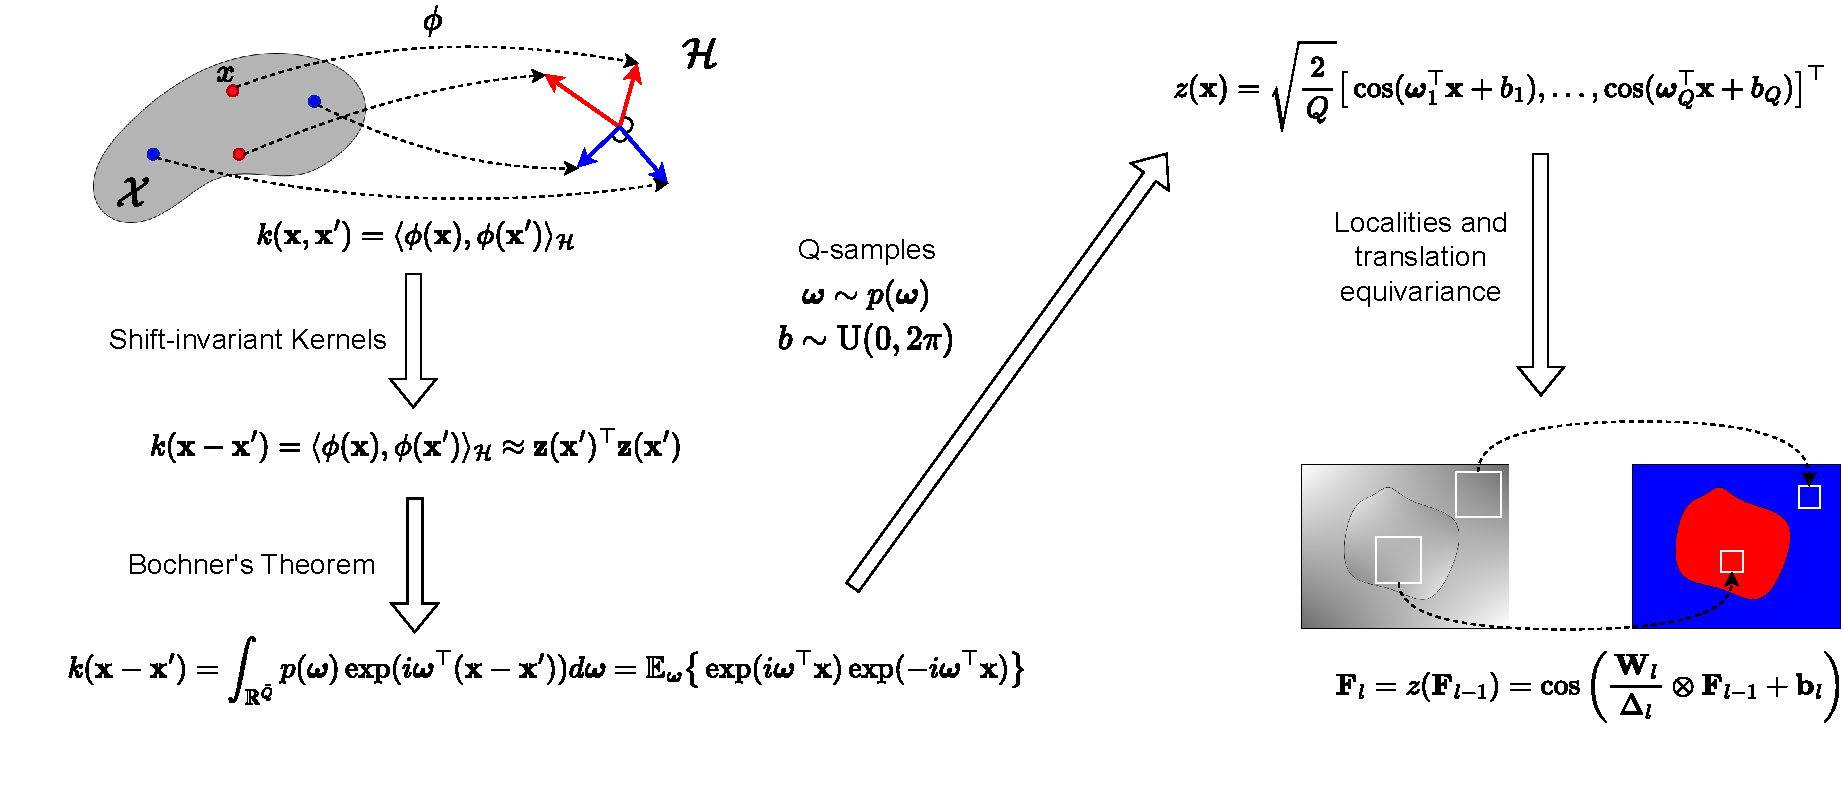
\includegraphics[trim={1.1cm 0 0 0},clip, width=0.95\textwidth]{Figures/CRFFg.pdf}
    \end{figure}
\end{frame}


\begin{frame}{Layer-Wise Weighted Class Activation Maps}

\begin{figure}
    \centering
    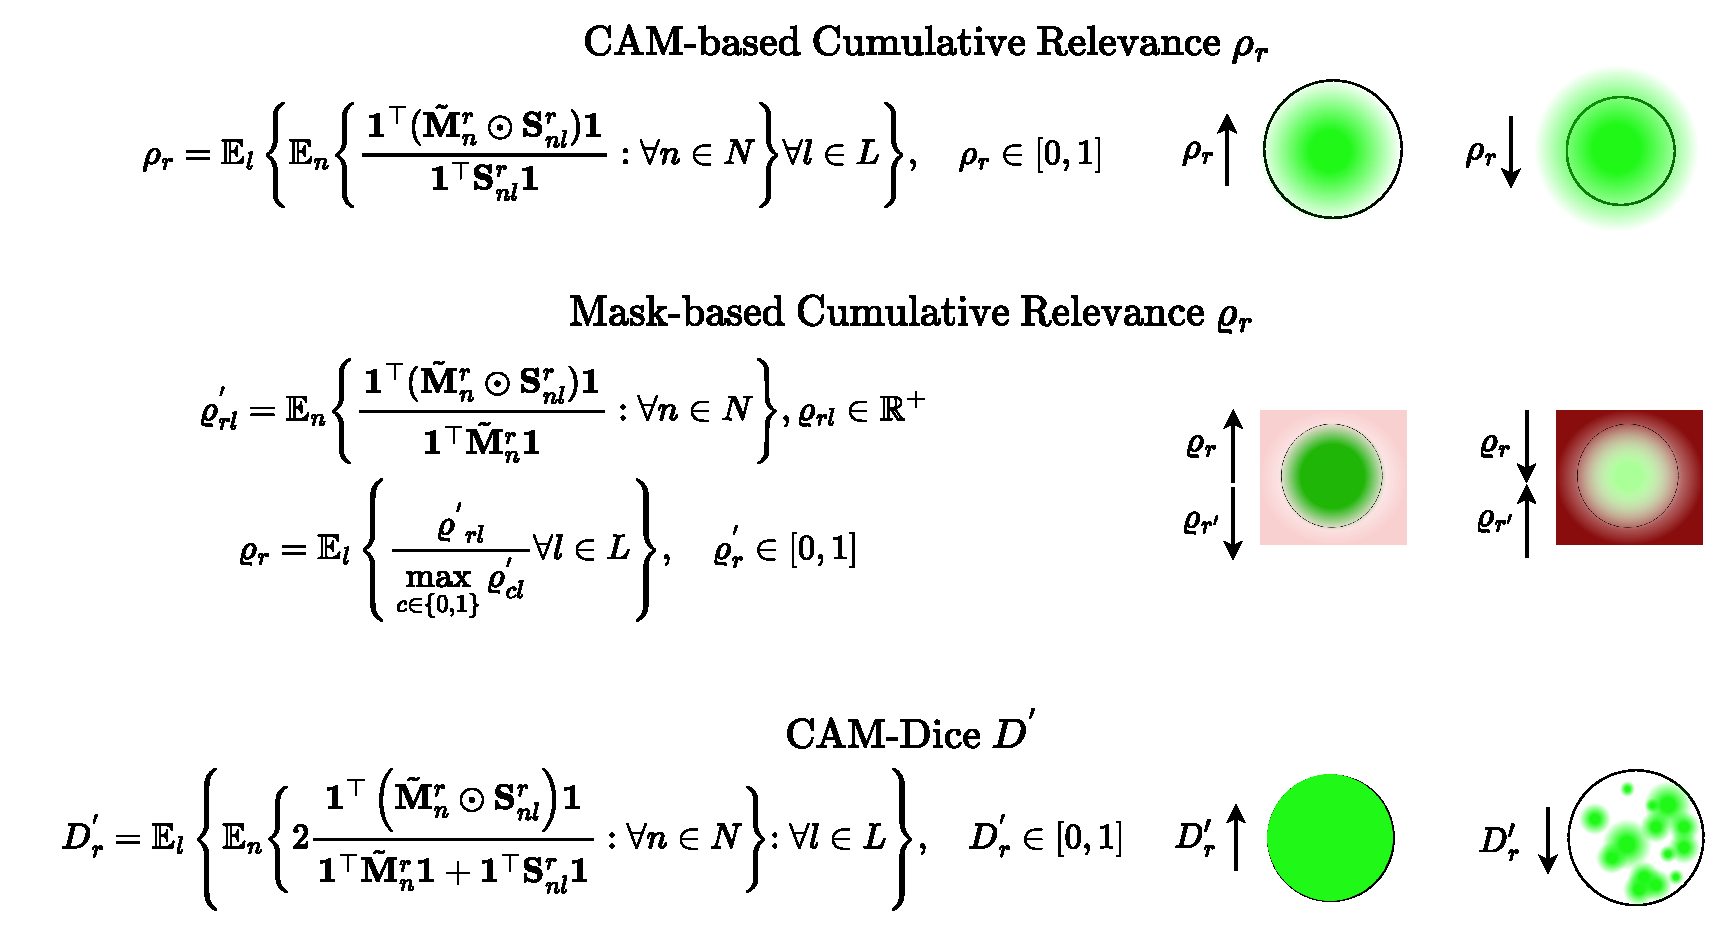
\includegraphics[width=0.8\textwidth]{Figures/camMeasures.pdf}

\end{figure}

\end{frame}

% \begin{frame}{Feet Semantic Segmentation}

% \begin{figure}
%     \centering
%     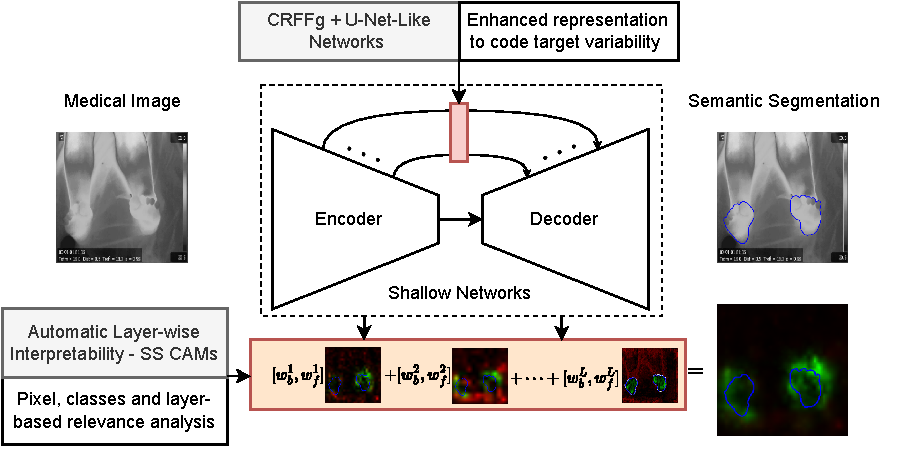
\includegraphics[width=0.935\textwidth]{Figures/aims_diagram.pdf}

% \end{figure}

% \end{frame}


\section{Experimental Set-up}

\begin{frame}{Dataset - ThermalFeet}
\begin{figure}
    \centering
    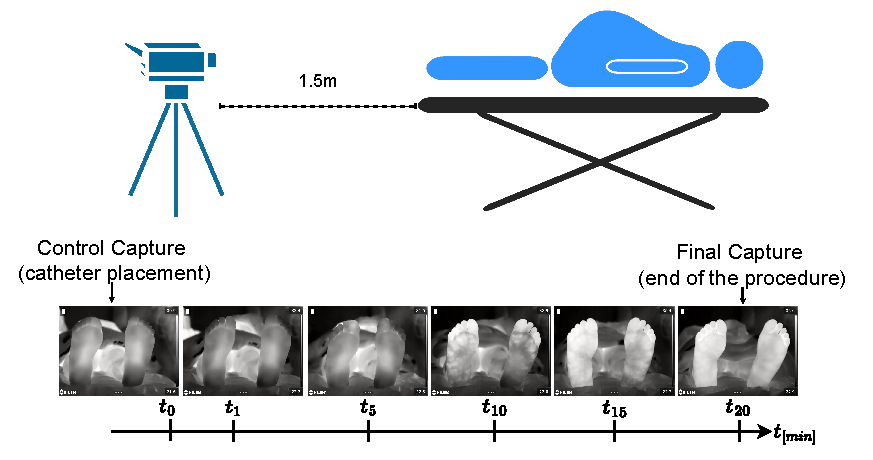
\includegraphics[width=0.7\linewidth]{Figures/camaraLocation.pdf}
\end{figure}
\begin{center}
    \textcolor{blue}{166 images, 80\% of the samples for training, 10\% for validation, and 10\% for testing.}\\ \textcolor{blue}{We test with and without data augmentation.}
\end{center}
\end{frame}


\begin{frame}{Method Comparison}

\vspace{-0.9cm}
\begin{columns}[t] % Align columns from the top
    \begin{column}{0.5\textwidth}
      \centering
      \begin{table}[htbp]
\centering
\caption{Variations for each Baseline Model (FCN, ResUNet, U-Net)}
\begin{tabular}{|l|l|l|l|}
\hline
Modification\textbackslash M           & No M  & M=1 & M=3 \\ \hline
Baseline   & x &     &     \\ \hline
CRFFg      &   & x   & x   \\ \hline
Stand Conv &   & x   & x   \\ \hline
\end{tabular}
\end{table}
    \end{column}

    \begin{column}{0.5\textwidth}
      \centering
      \begin{figure}
          \centering 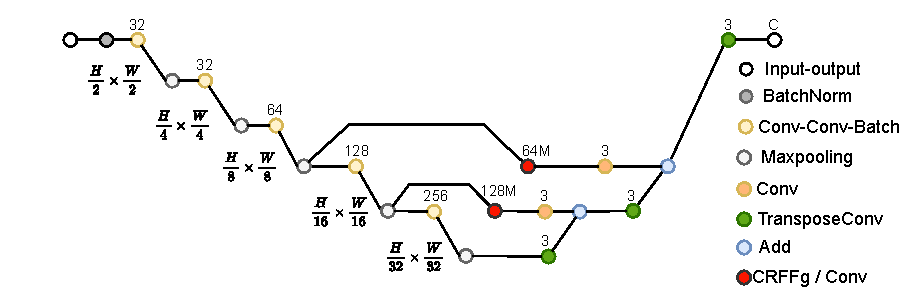
\includegraphics[width=0.98\textwidth]{Figures/fcn_arch.pdf}
          \caption{FCN Architecture}
      \end{figure}
    \end{column}
  \end{columns}

  %\vspace{1em} % Add some space between rows

  \begin{columns}[t] % Align columns from the top
    \begin{column}{0.5\textwidth}
      \centering
      \begin{figure}
          \centering 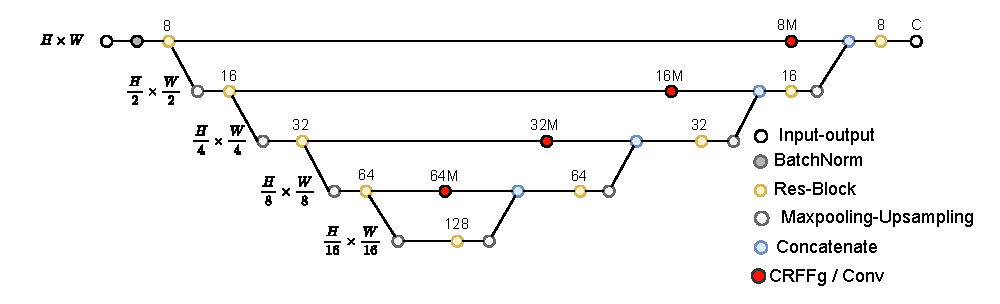
\includegraphics[width=1\textwidth]{Figures/res_unet_arch.pdf}
          \caption{ResUNet Architecture}
      \end{figure}
    \end{column}

    \begin{column}{0.5\textwidth}
      \centering
      \begin{figure}
          \centering 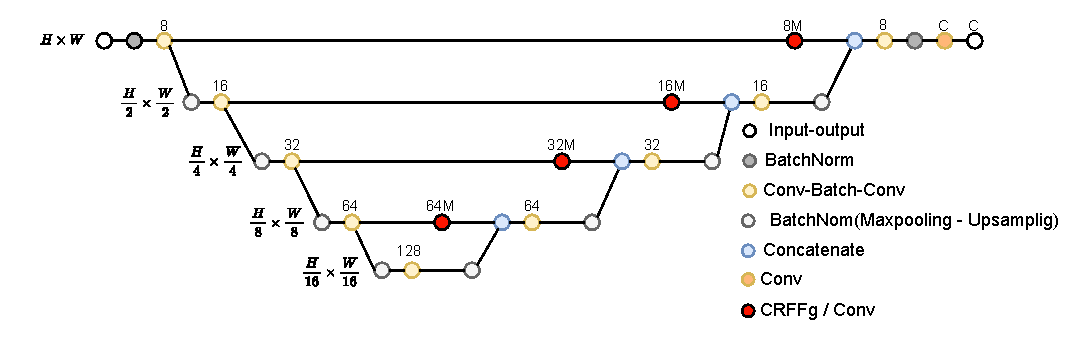
\includegraphics[width=1\textwidth]{Figures/unet_arch.pdf}
          \caption{U-Net Architecture}
      \end{figure}
    \end{column}
  \end{columns}




\end{frame}



\begin{frame}{Performance Measures}

    
\begin{columns}


\column{0.5\textwidth}

\begin{itemize}
    \setlength\itemsep{1em}
    \item $\text{Dice}[\%] = 100 \frac{2|\mathbf{M}  \cap \mathbf{\hat{M}} |}{|\mathbf{M} | + |\mathbf{\hat{M}} |} = 100\frac{2 TP}{2TP + FP + FN}$
    
    
    \item $\text{Jaccard}[\%] = 100\frac{|\mathbf{M}  \cap \mathbf{\hat{M}} |}{|\mathbf{M}  \cup \mathbf{\hat{M}} |} = 100\frac{TP}{FN + FP + TP} $\\
    
    \item $\text{Sensitivity}[\%] = 100\frac{TP}{TP + FN}$

    \item $\text{Specificity}[\%] = 100\frac{TN}{TN + FP}$

    \item $\text{Precision}[\%] = 100\frac{TP}{TP + FP} $

\end{itemize}
\column{0.5\textwidth}
 \begin{figure}
     \centering 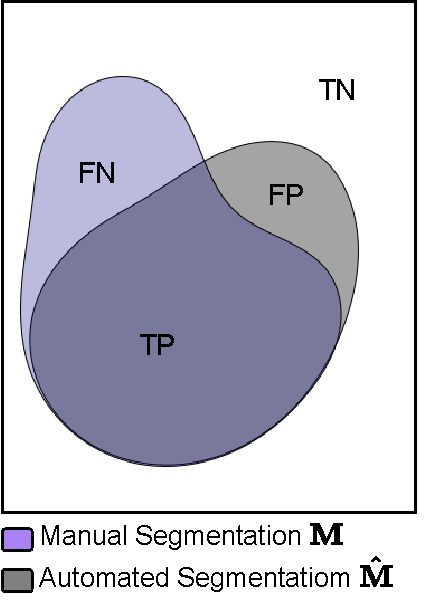
\includegraphics[width=0.6\linewidth]{Figures/regions.pdf}
     %\label{}
 \end{figure}
\end{columns}    

    
\end{frame}


\section{Results}



\begin{frame}{Visual Inspection Results}

\begin{figure}
    \centering
    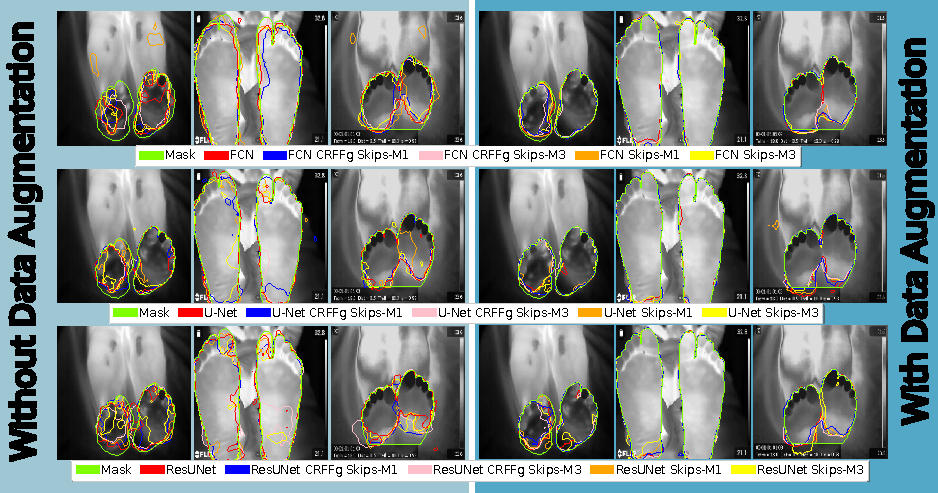
\includegraphics[width=0.87\linewidth]{Figures/visual_inspection.pdf}
\end{figure}

\end{frame}

\begin{frame}{Quantitative Semantic Segmentation Results}
    \begin{figure}
        \centering 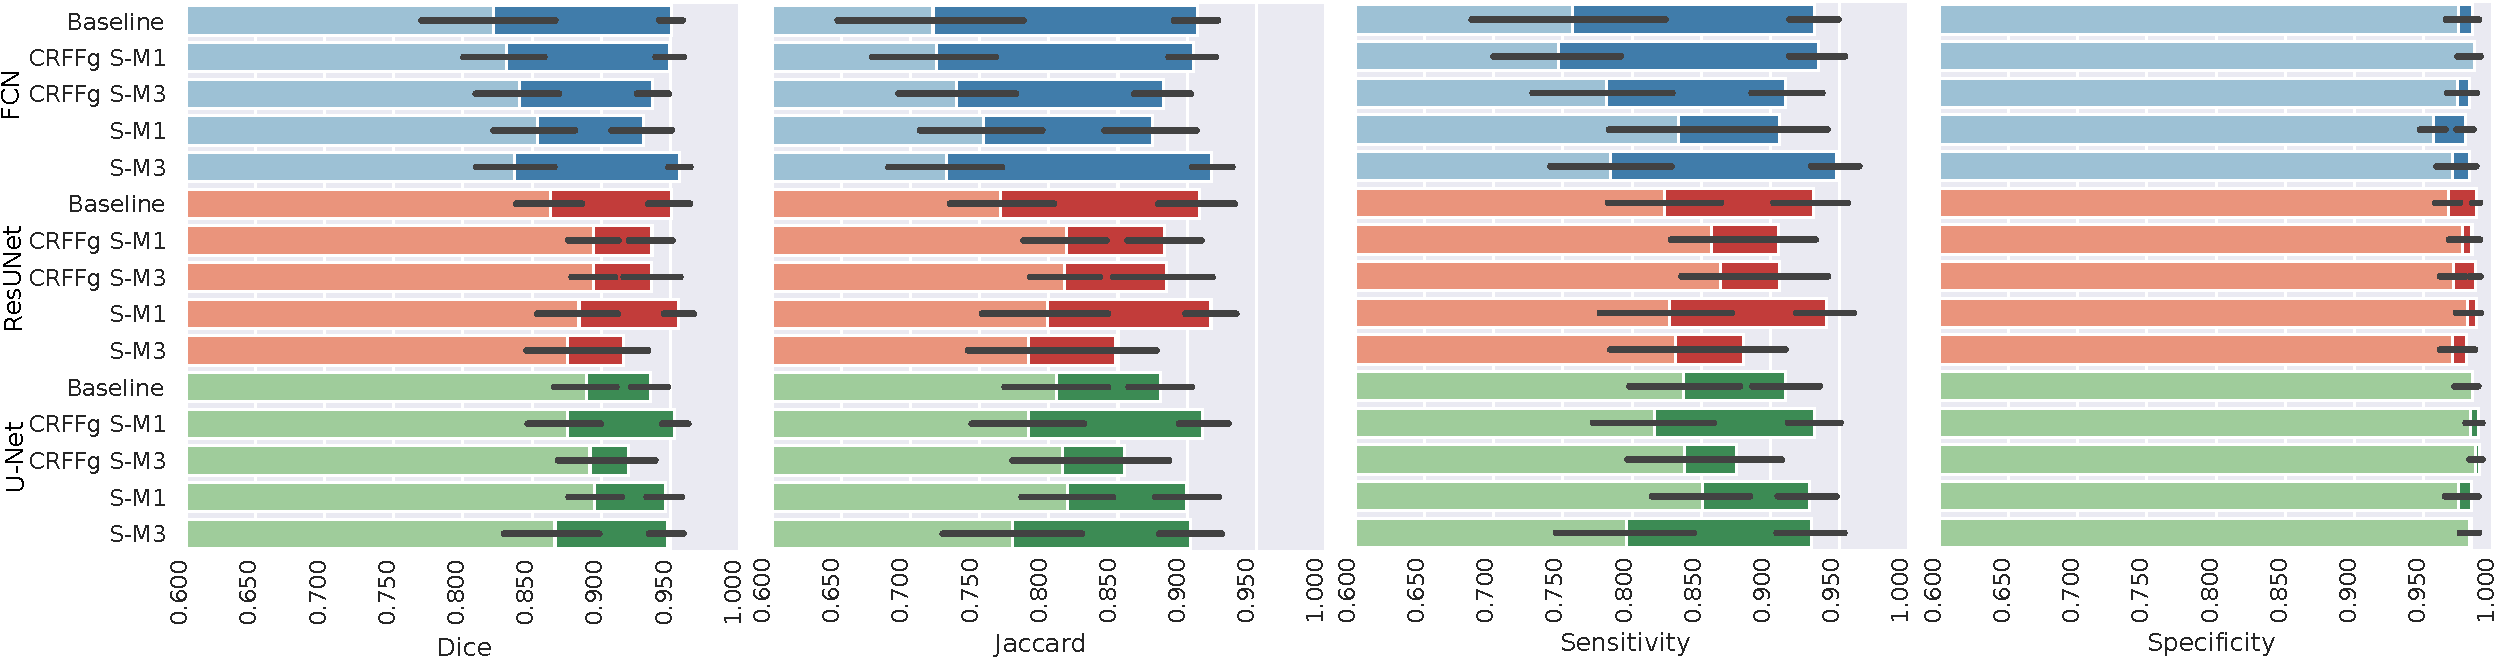
\includegraphics[width=1\linewidth]{Figures/results_infrared_thermal_feet.pdf}
    \end{figure}
    \begin{figure}
        \centering 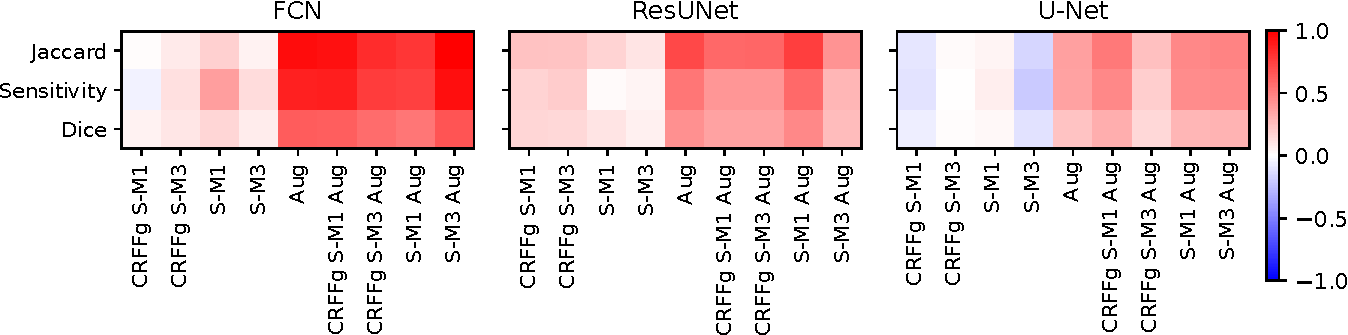
\includegraphics[width=0.695\linewidth]{Figures/baseline_models.pdf}
    \end{figure}
\end{frame}

\begin{frame}[allowframebreaks]{Interpretability Results}

\begin{figure}
    \centering
    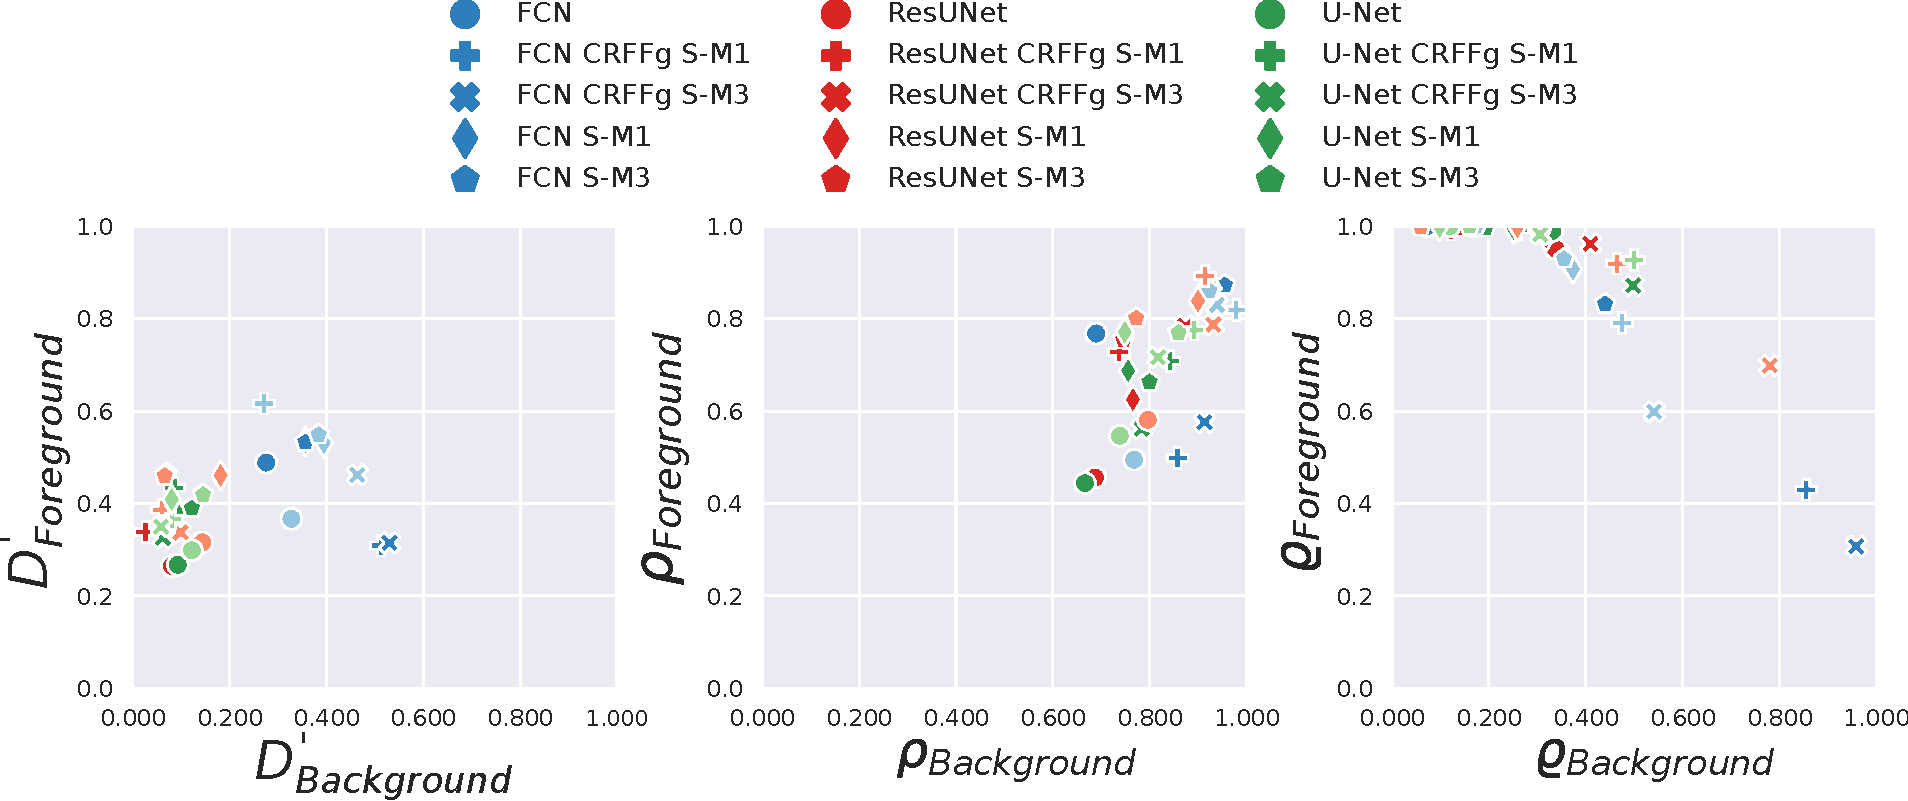
\includegraphics[width=1\linewidth]{Figures/interpretability_results_infrared_thermal_feet.pdf}
\end{figure}
\framebreak
\begin{figure}
    \centering
    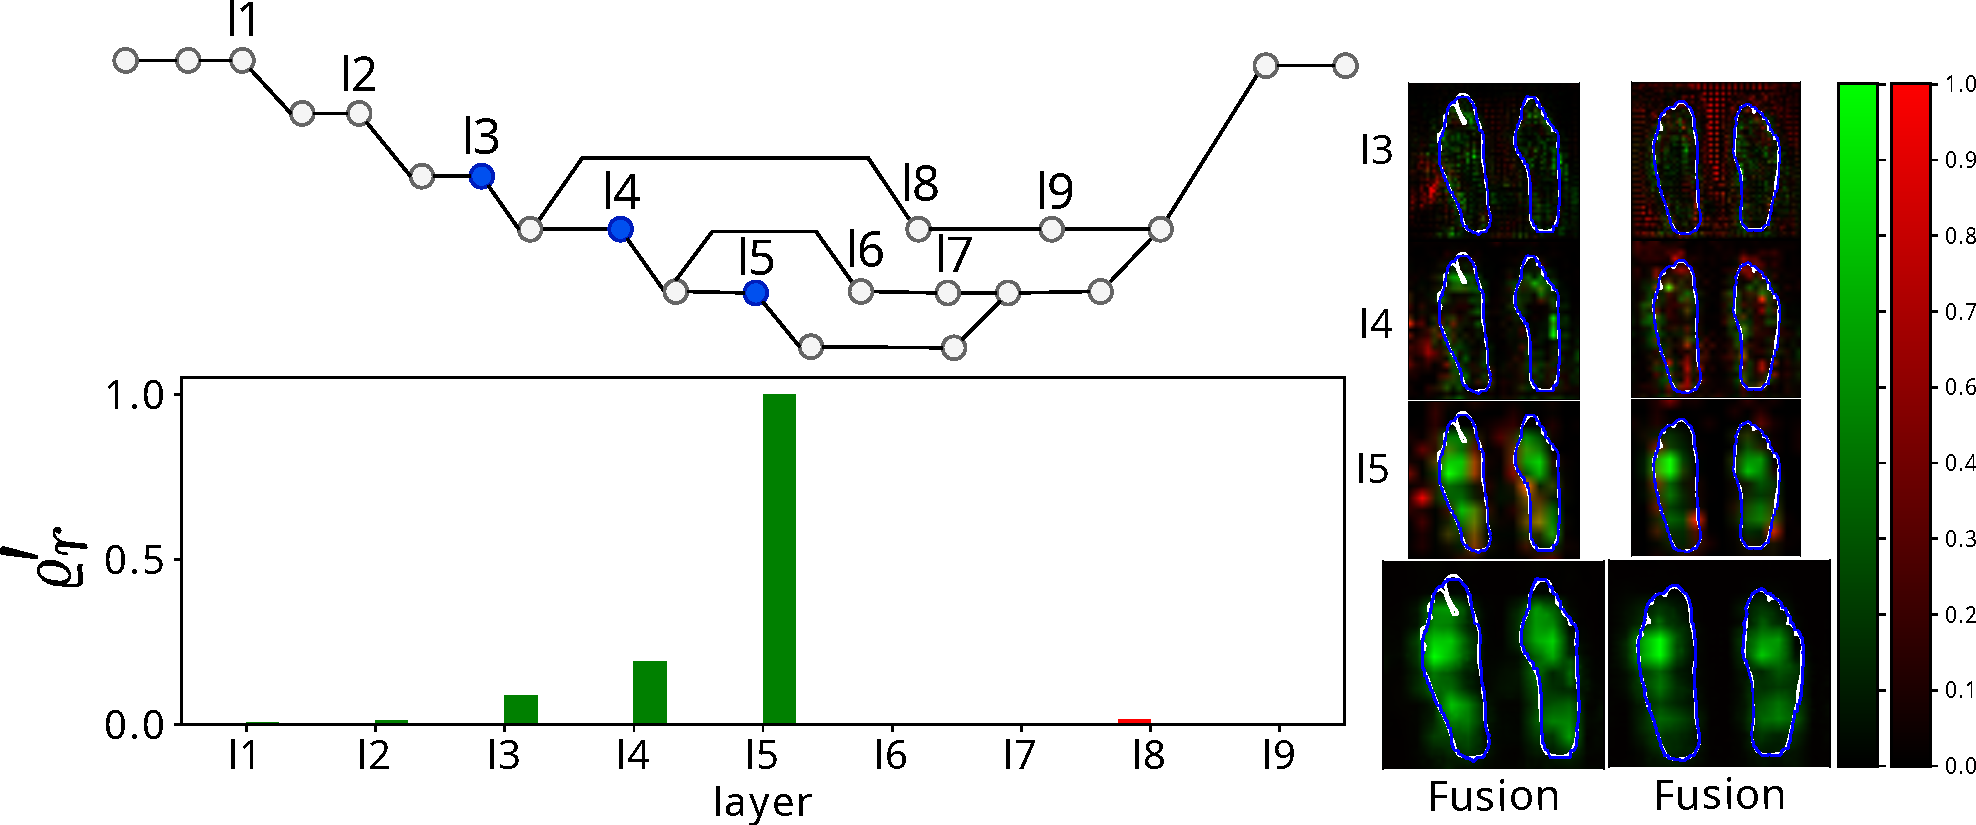
\includegraphics[width=0.89\linewidth]{Figures/fcn_best.pdf}
    \caption{FCN CRFFg S-M3 without data Augmentation}
\end{figure}
\framebreak

\begin{figure}
    \centering
    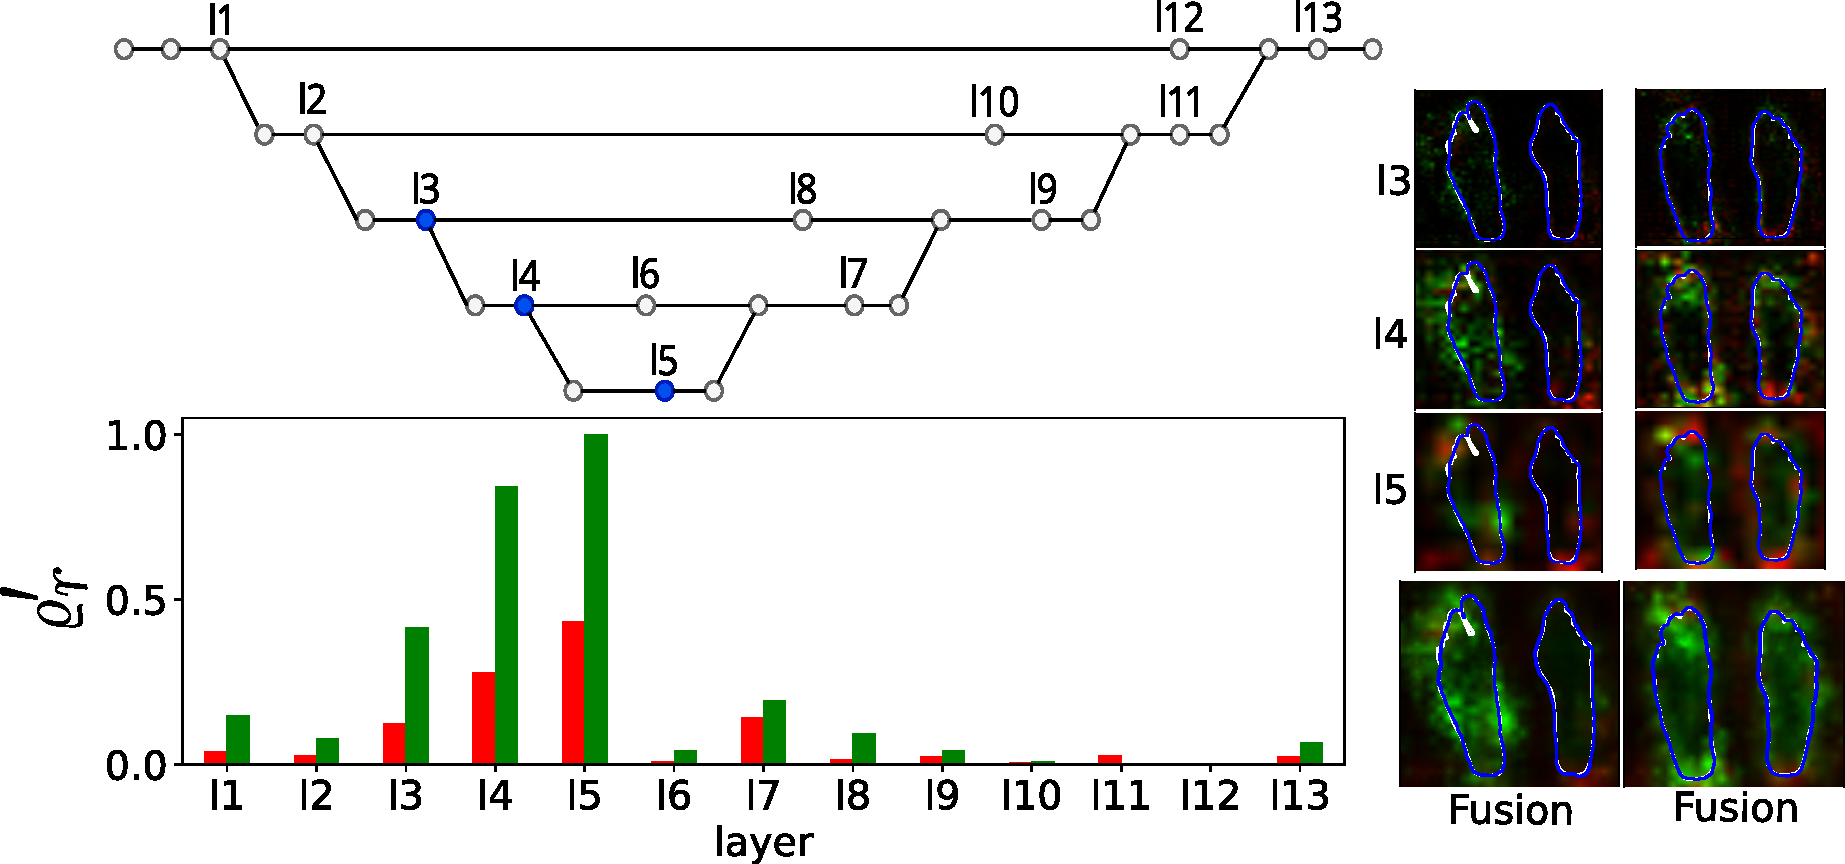
\includegraphics[width=0.79\linewidth]{Figures/resunet_best.pdf}
    \caption{ResUNet CRFFg S-M3 without data Augmentation}
\end{figure}
\framebreak

\begin{figure}
    \centering
    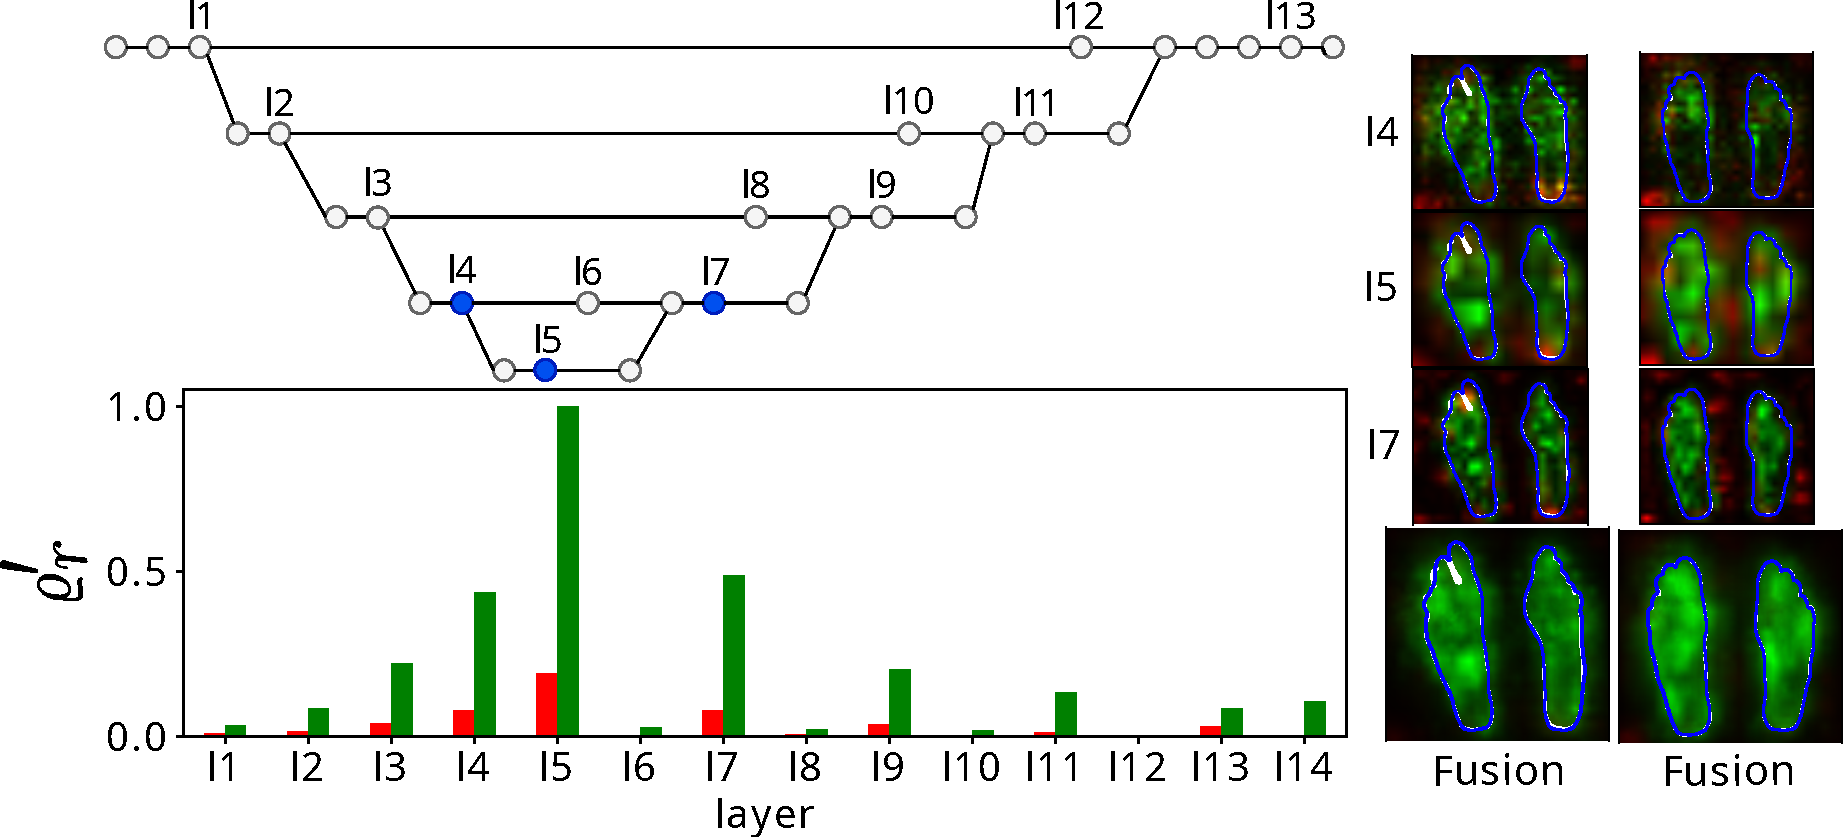
\includegraphics[width=0.79\linewidth]{Figures/unet_best.pdf}
    \caption{U-Net CRFFg S-M3 with data Augmentation}
\end{figure}

\end{frame}



\begin{frame}{Integration into a software tool for medical use}
\begin{figure}
        \centering
        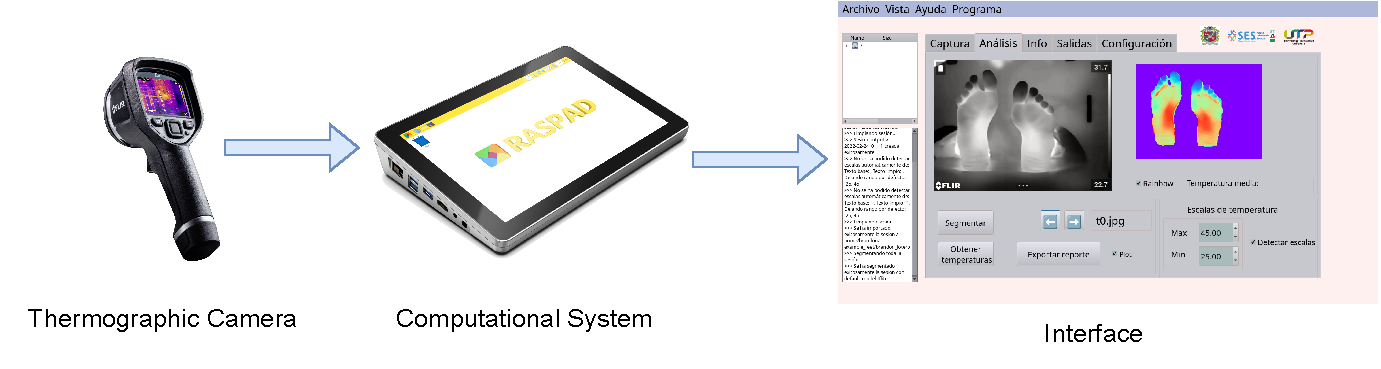
\includegraphics[width=0.98\linewidth]{Figures/system.pdf}
        \caption{Monitoring system for temperature changes in feet soles able to work in obstetrics environment (easy to use for the medical staff).}
        % \label{}
\end{figure}
    
\end{frame}



\begin{frame}{Integration into a software tool for medical use}
\begin{figure}
        \centering
        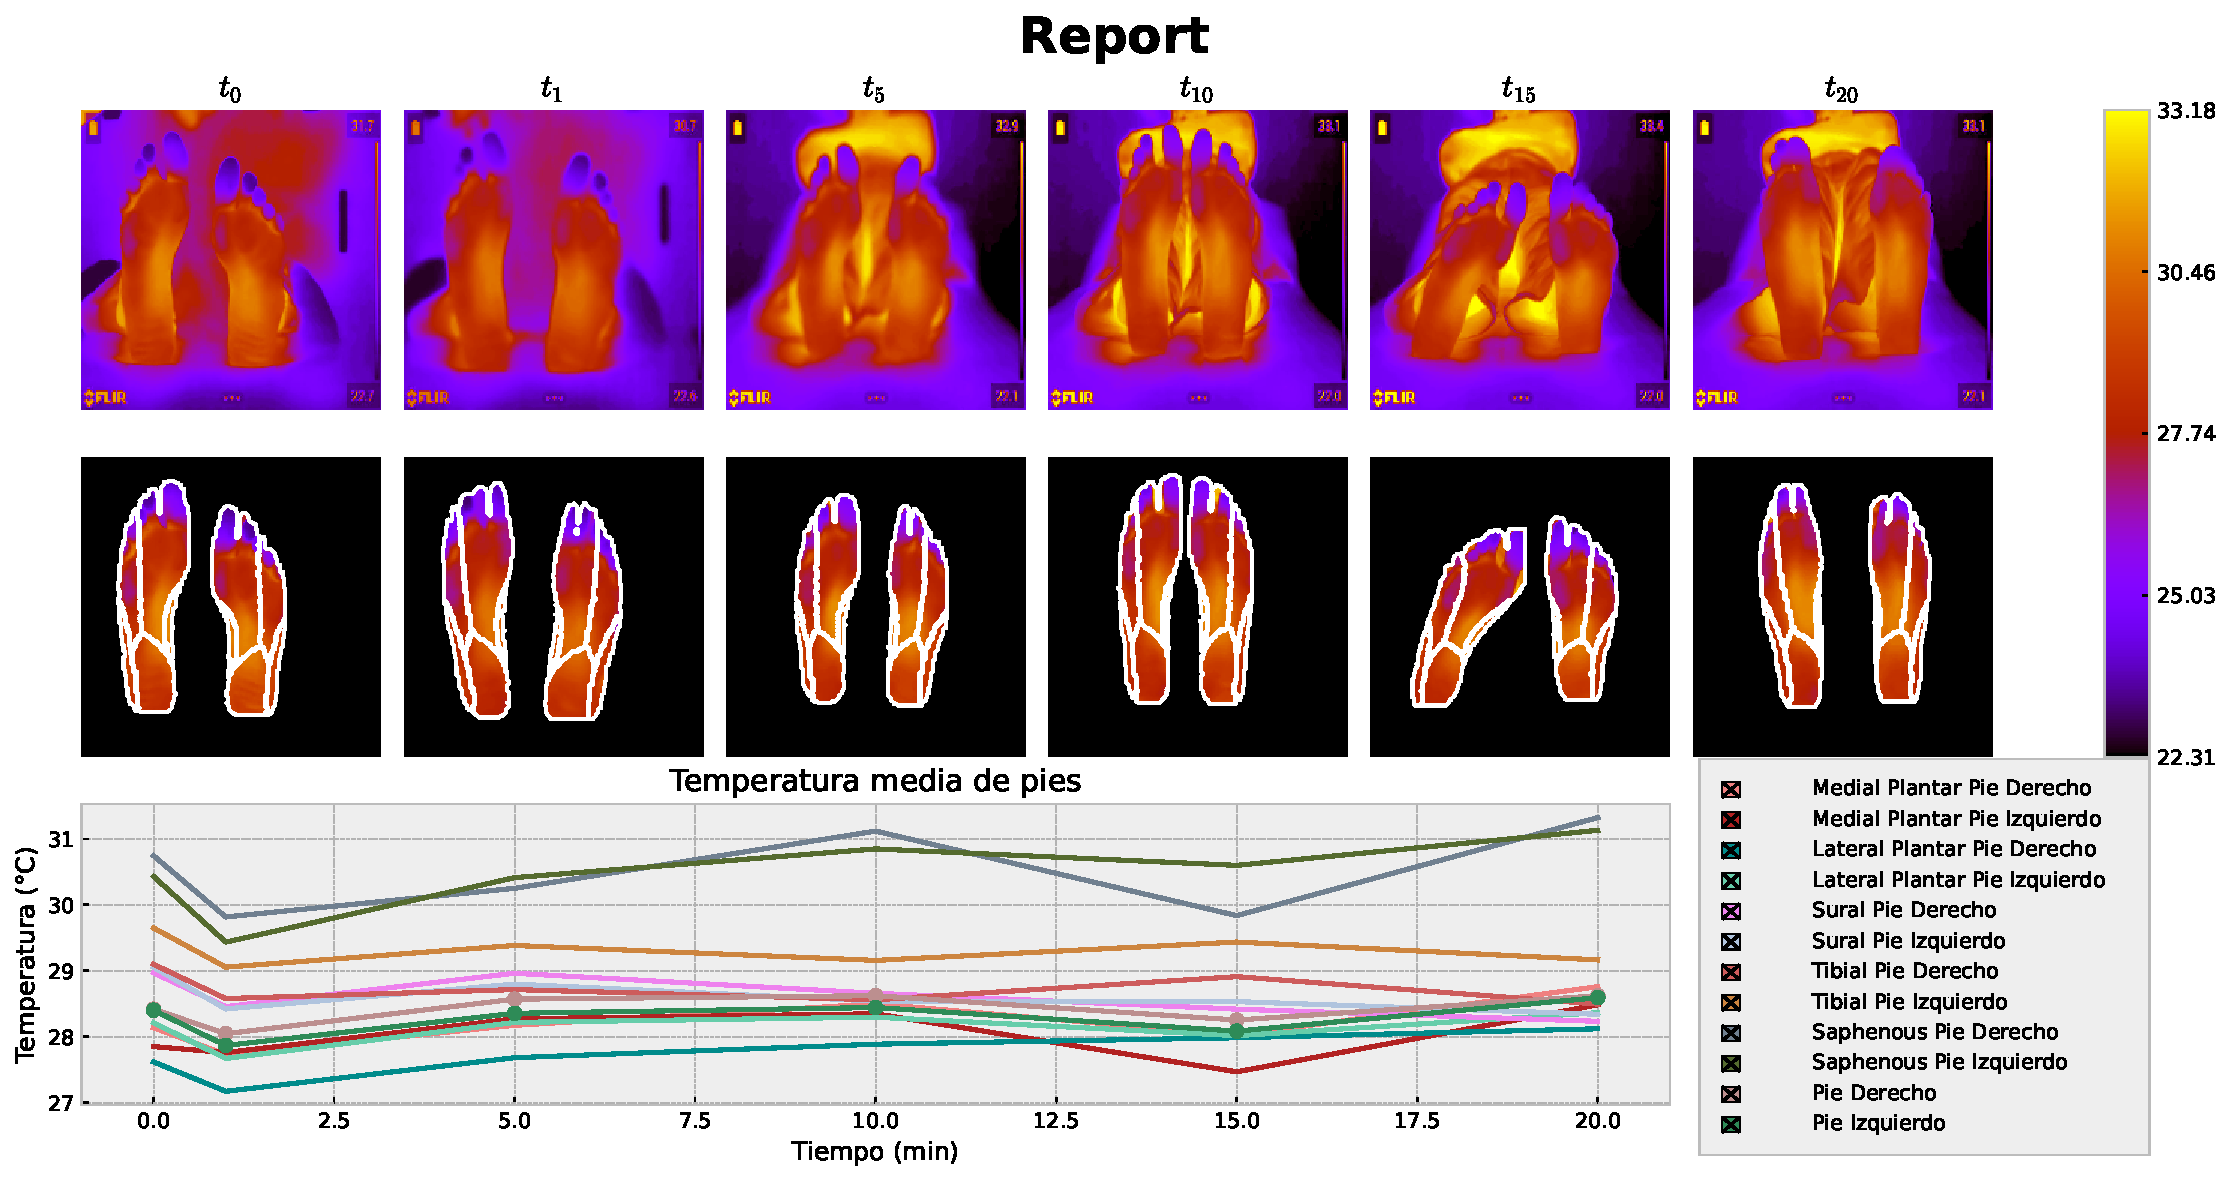
\includegraphics[width=0.87\linewidth]{Figures/report.pdf}
        % \caption{Data adquisition timeline}
        % \label{}
\end{figure}
    
\end{frame}



\section{Conclusions}

\begin{frame}{Conclusions}

\begin{itemize}
    \setlength\itemsep{1em}

        \item We propose an extension of the Random Fourier Features tailored for spatial data, introducing CRFFg—a data-driven approach that leverages gradient descent. 
        
        \item Our innovative extension effectively enhances feature representation within the skip connection of encoder-decoder models, particularly for semantic segmentation tasks. 
    
    \item We tested 15 model variations of three well-known  deep learning architectures for automatic feet semantic segmentation on thermal images that exhibit small sample size and high variability of regions of interest.
    


    \item We have introduced quantitative measures for enhancing interpretability in semantic segmentation models used in the medical field. 
    
    \item Our approach quantifies the relevance location of specific regions, the sensibility across multiple regions of interest, and their homogeneity.
\end{itemize}


\end{frame}

\begin{frame}{Future Work}

\begin{itemize}
    \setlength\itemsep{1em}
    \item Analyzing the spectral representation of the CRFFg to gain insights into underlying patterns, leading to a deeper understanding and potential improvements \cite{ZHANG202041}.
    
    \item Incorporating Bayesian approximation techniques to quantify uncertainties, model relationships between variables more accurately, and potentially uncover new strategies related to our CRFFg layer \cite{MILLER2022100598}.
    
    \item Employing regularization techniques to mitigate overfitting using the proposed interpretability measures \cite{chang2020mixupcam, 9506582}.
\end{itemize}



\end{frame}

\begin{frame}{Acknowledgments}

\begin{itemize}
    \item \textit{``Herramienta de apoyo a la predicción de los efectos de anestésicos locales vía neuroaxial epidural a partir de termografía por infrarrojo" (Code 111984468021)} funded by MINCIENCIAS
    \item \textit{``Sistema prototipo de visión por computador utilizando aprendizaje profundo como soporte al monitoreo de zonas urbanas desde unidades aéreas no tripuladas" (Hermes Code 55261)}, funded by Universidad Nacional de Colombia.
\end{itemize}



\begin{center}
	{\large{\textbf{\textcolor[rgb]{0.00,0.00,1.00}{Thank you!}}}}\\
	\vspace{0.1cm}
	 Juan Carlos Aguirre Arango\\ \scriptsize{jucaguirrear@unal.edu.co}
\end{center}    
    
\end{frame}




\begin{frame}[allowframebreaks]
\frametitle{References}
{\tiny 
\bibliographystyle{apalike}
\bibliography{References, References1}
}
\end{frame}




\end{document}

